\documentclass[a4paper,openright, 14pt]{article}
\usepackage[utf8]{inputenc}
\usepackage{rotating, graphicx}
\usepackage{tikz}
\usetikzlibrary{datavisualization}
\usetikzlibrary{datavisualization.formats.functions}

\graphicspath{ {./images/} }

\usepackage{fullpage}
\newcommand{\ssection}[1]{%
\section[#1]{\centering\normalfont\scshape #1}}
\newcommand{\ssubsection}[1]{%
\subsection[#1]{\bfseries\normalfont\scshape #1}}
\newcommand{\ssubsubsection}[1]{%
\ssubsubsection[#1]{\bfseries\normalfont\scshape #1}}

\title{The Bee Problem}
\author{Lauren Bourque}
\date{February 4, 2019}

\begin{document}

\maketitle
\begin{center}
    
\includegraphics[width=4cm, height=4cm]{Images/bee.png}
\end{center}
\section*{The Problem}
A bee starts at point $P_0$, flies to point $P_1$, and lands there. The bee then returns half of the way to $P_0$, landing at $P_2$. The bee returns half of the way to $P_1$, landing at $P_3$, and so forth.\\
1. Predict the bee's ultimate location.\\
2. Predict the bee's ultimate location if on each trip, it returns one-third of the way to the previous point instead of one-half of the way.\\
3. Predict the bee's ultimate location for one-fourth of the way.\\
4. Generalize the problem by predicting the bee's ultimate location for one-kth of the way.
\section*{Introduction: Visualizing the Flight}
Before we try to write out an equation for the first bee's flight, let's draw a visual to help us better understand his flight path.
\begin{center}
    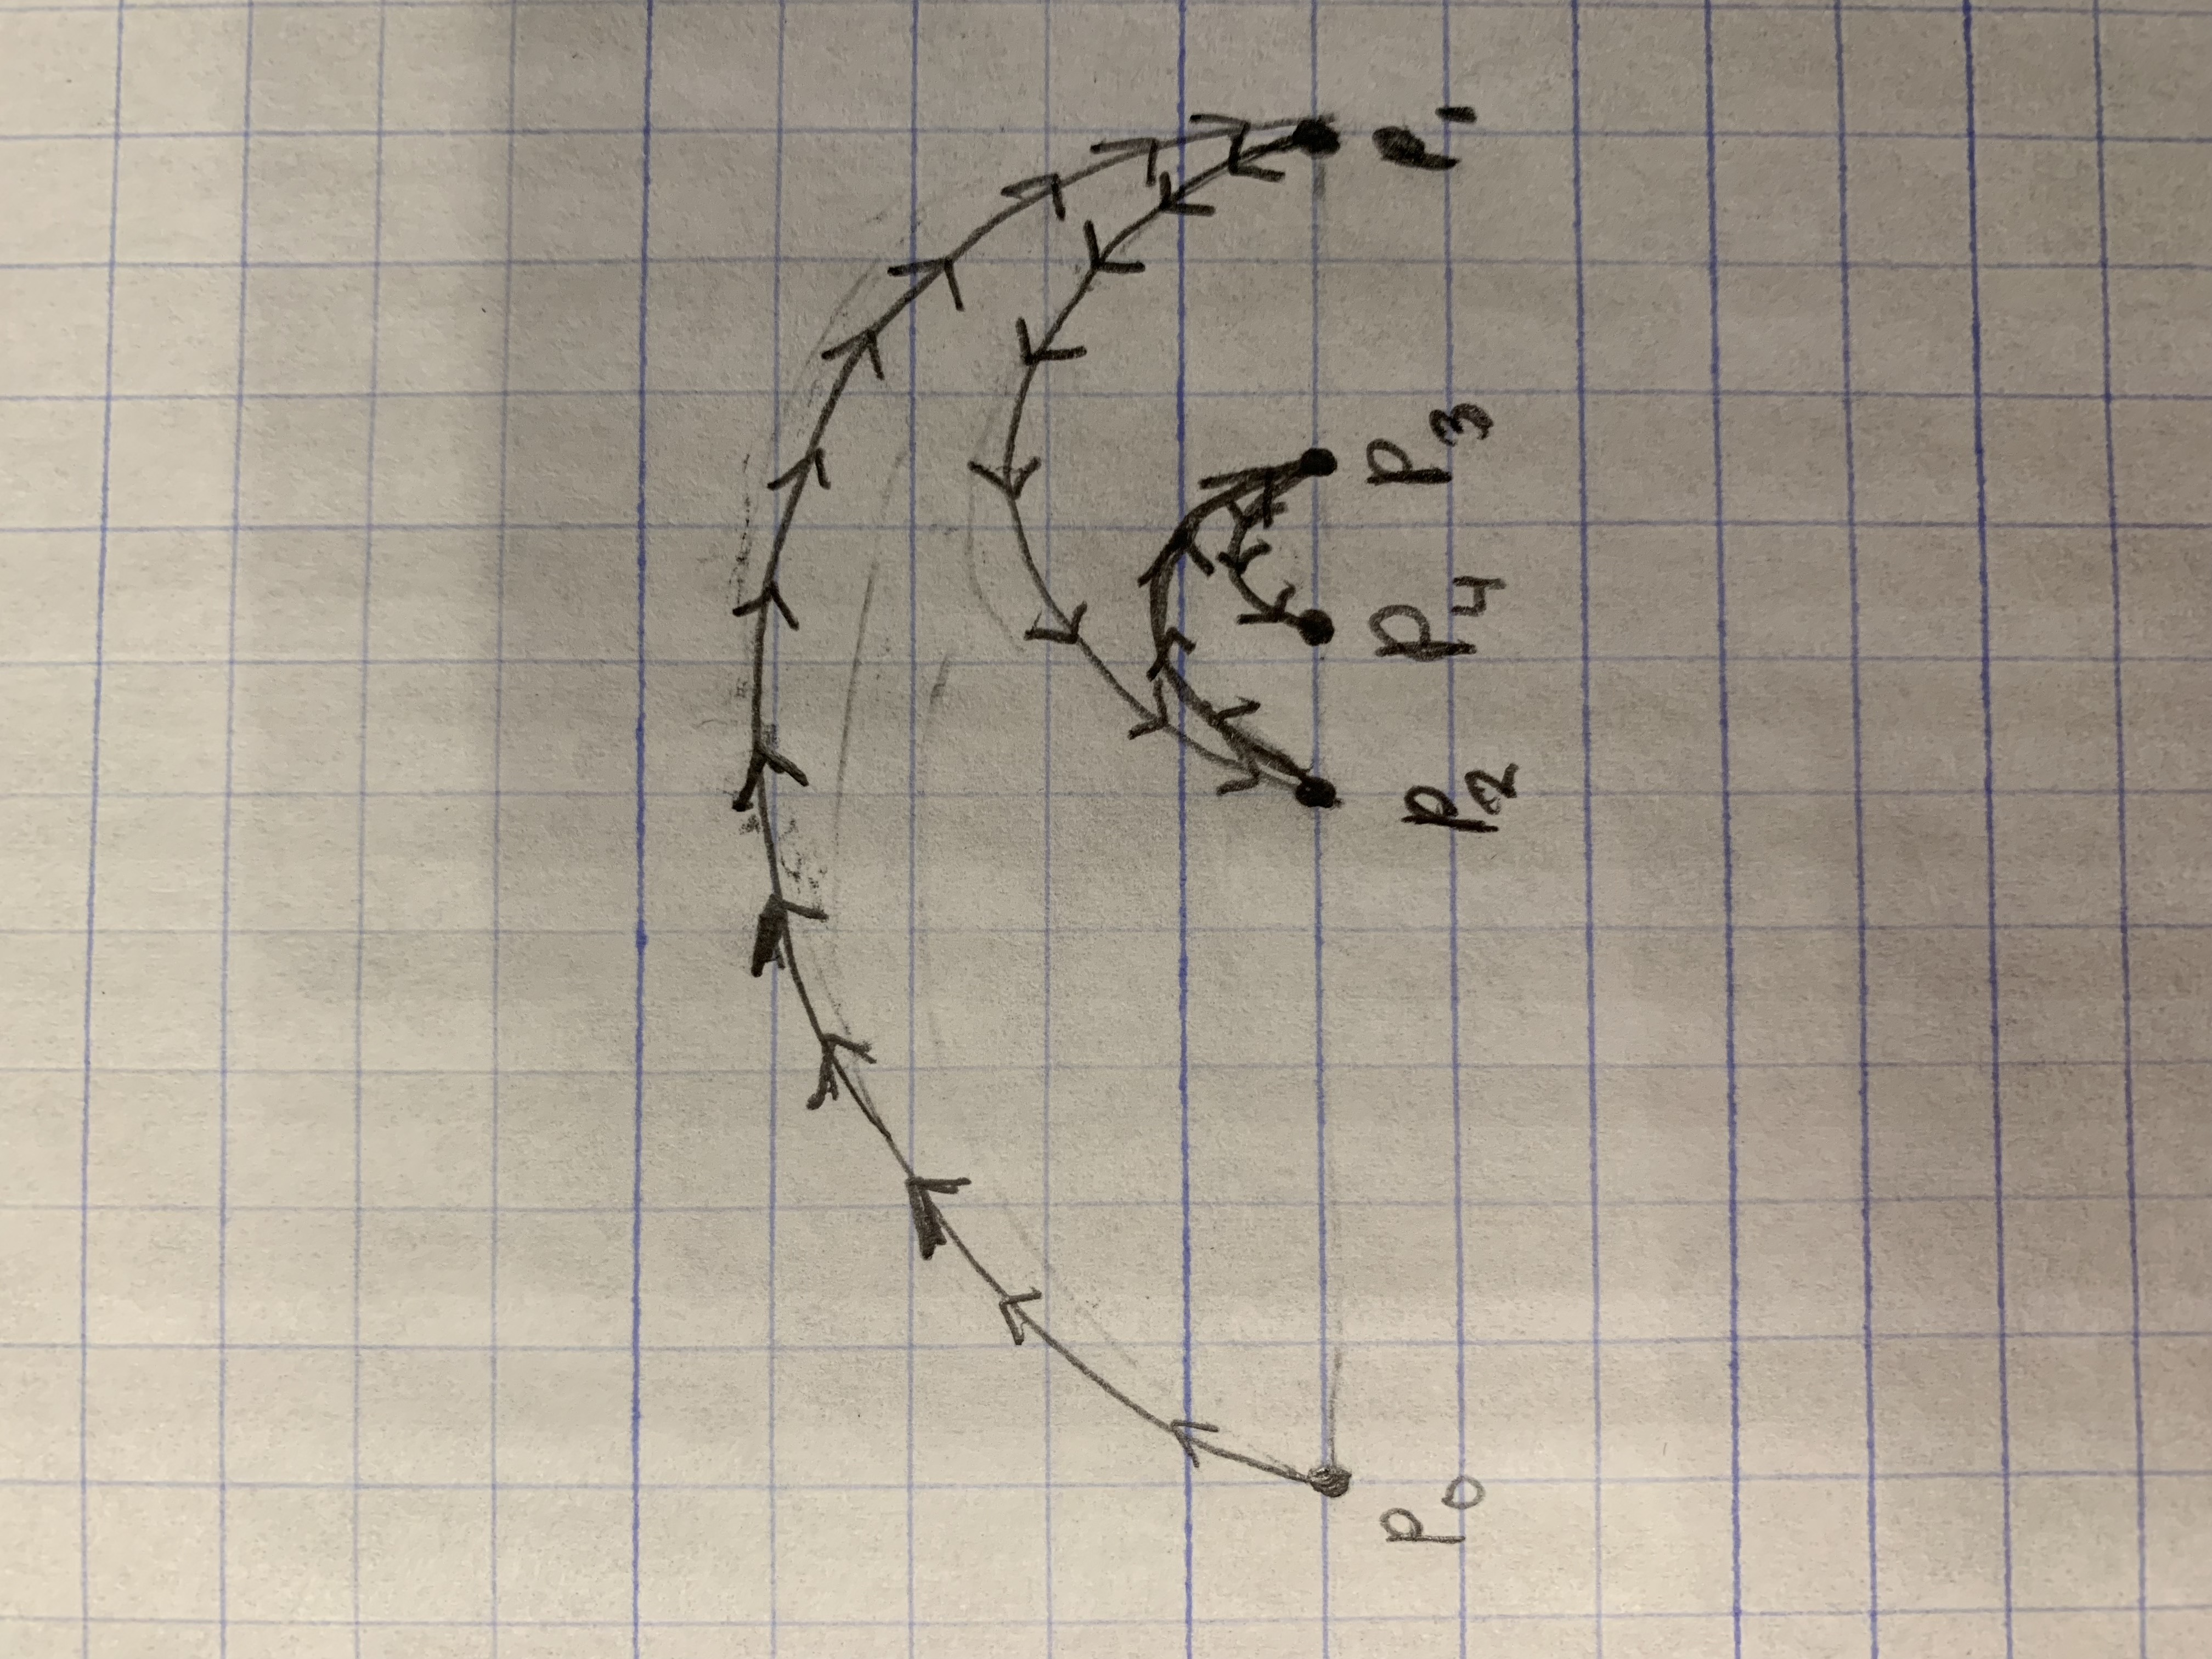
\includegraphics[angle=270, width=4cm ]{Images/path.jpg}
\end{center}
As we can see here, the image is labeled with arrows pointing in the bee's direction of flight. We can see that the bee is flying from point to point. Each point that the bee stops at appears to be getting closer and closer to the point before. Let's create a table of values of the distance from $P_0$ at several points so that we can try to recognize a pattern.
\section*{Finding a Pattern}
\begin{tabular}{c|c}
Point & Distance from $P_0$\\
    \hline
    $P_1$ & 1 \\
    \hline
    $P_2$ & $\frac{1}{2}$ \\
    \hline
    $P_3$ & $\frac{3}{4}$ \\
    \hline
    $P_4$ & $\frac{5}{8}$
\end{tabular}
\\
If we look at the difference between $P_1$ and $P_2$, we can see that $\frac{1}{2}$ was subtracted. If we look at the difference between $P_2$ and $P_3$, we can see that $\frac{1}{4}$ was added. If we look at the difference between $P_3$ and $P_4$, we can see that $\frac{1}{8}$ was subtracted.\\\\
Let's look at the change in differences between consecutive points. We can see that the difference between $P_1$ and $P_2$ is -$\frac{1}{2}$, which can be rewritten as -$\frac{1}{2^1}$. This change was added to $P_1$ to give us $P_2$. If we look the difference between $P_2$ and $P_3$, we can see that $\frac{1}{4}$ was added to $P_2$, which can be rewritten as $\frac{1}{2^2}$. If we look at the difference between $P_3$ and $P_4$, we can see that -$\frac{1}{8}$ was added to $P_3$, which can be rewritten as -$\frac{1}{2^3}$. From this, we can begin to see a pattern. So what is it?\\\\
The differences switch from being positive to negative. There's always a one in the numerator and 2 to some power in the denominator. Since the difference is always being added to the previous term which was also added to the previous term and so on, we want to try to write this as a series, or a sum of terms in a sequence. Then, we can use our knowledge of series to discover which point the buzzing bee will approach if it continues to fly infinitely. 
\section*{Creating a Series}
Since we've discovered that the difference between terms is -$\frac{1}{2}$ to some power, let's incorporate that into our series.
$$\sum\limits_{k=0}^{\infty} (-\frac{1}{2})^k$$
We want to start our summation at k=0 since the first distance from $P_0$ is one and anything to the zeroth power is 1. Let's try looking at the terms up to k=3. Then, we'll sum these terms and see if they match our calculated distance from $P_0$ of $\frac{5}{8}$. 
$$1+(-\frac{1}{2})^1+(-\frac{1}{2})^2+(-\frac{1}{2})^3$$
Which equals
$$1-\frac{1}{2}+\frac{1}{4}-\frac{1}{8}$$
Let's get a common denominator and add these together.
$$\frac{8}{8}-\frac{4}{8}+\frac{2}{8}-\frac{1}{8}=\frac{5}{8}$$
Eureka! Our series worked. Now let's use our knowledge of series to try and figure out what the series will converge to, or where the bee will end up infinitely flying closer towards. We can recognize this as a geometric series, -$\frac{1}{2}$ is to the kth power, making it a common ratio between terms. Let's try to derive the geometric series so we fully understand where it comes from.
$$\fbox{\textbf{Time for a Quick Break! Fun Fact:} Honey bees beat their wings 200 times per second.}$$
\section*{Deriving the Geometric Series Formula}
So, we know that a geometric series can be written as 
$$S_n=a+ar+ar^2+ar^3...+ar^{n-1}$$
where a is the first term and r is the common ratio. Let's try multiplying the series by r to see the changes that are made.
$$r\cdot S_n=ar+ar^2+ar^3+ar^4...+ar^{n-1}+ar^{n}$$
By looking at this, we can see that some terms would cancel out if we subtracted $S_n$ from $r\cdot S_n$. The only thing that would be left would be $ar^n-a$
$$r\cdot S_n-S_n=ar^n-a$$
Let's try to isolate $S_n$
$$S_n(r-1)=ar^n-a$$
$$S_n=\frac{ar^n-a}{r-1}$$
Now, let's take the limit as n approaches infinity of this, so that we can get a formula to find what a geometric series converges to.
$$\lim_{x\to\infty} \frac{a(r^n-1)}{r-1}$$
Now, we have to set bounds for r so that the series will be able to converge. We know that r can't equal 1 because it would create a number over 0, which is undefined. We also know that it can't be larger than one because that would create a number to the infinite power which would diverge and not give us the convergence that we want. The same goes for a number less than negative one. Therefore, the bounds for the equation are:
$$-1<r<1$$
If r is between these numbers, it would have to be a fraction. A fraction to the infinite power eventually converges to 0 so we can substitute 0 in for $r^n$.
$$\frac{a(0-1)}{r-1}=-\frac{a}{r-1}=\frac{a}{1-r}$$
So, we know that
$$\lim_{x\to\infty} =\frac{a}{1-r}$$
This is the formula that will allow us to find what geometric series converge to.
\section*{Finding the Bee's Ultimate Location (Series Convergence)}
Since we know that a is the first term and r is the common ratio in a geometric series, we need to identify those values for our series.
$$\sum\limits_{k=0}^{\infty} (-\frac{1}{2})^k$$
In this series, a would be $1$ and the common ratio would be $-\frac{1}{2}$. Let's substitute these values into the equation.
$$\lim_{k\to\infty}\sum\limits_{k=0}^{\infty} (-\frac{1}{2})^k= \frac{1}{1--\frac{1}{2}}=\frac{1}{\frac{3}{2}}=\frac{2}{3}$$
So, the bee's ultimate location would be $\frac{2}{3}$ of the distance from $P_0$. Let's confirm this by looking at a visual.
\begin{center}
    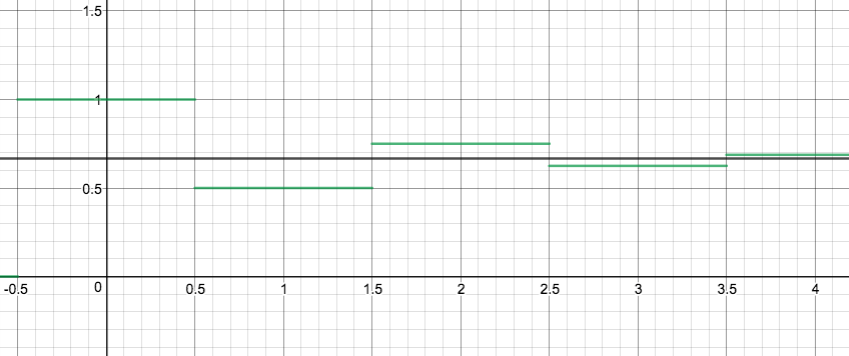
\includegraphics[width=7cm, height=4cm]{Images/line.png}
\end{center}
As we can see here, the line $\frac{2}{3}$ is graphed as the horizontal black line. The small lines approaching it are the partial sums of the equation. For example, the line at x=0 is the distance between $P_0$ and $P_1$, the line at x=1 is the distance between $P_1$ and $P_2$, the line at x=2 is the distance between $P_2$ and $P_3$, and so on. We can see that the partial sums start above the horizontal line and then switch between below and above, infinitely. This represents the switch between positive and negative values in the series. The partial sums are growing closer and closer to $\frac{2}{3}$, approaching from above and below. This means that $lim_{k\to\infty}\sum\limits_{k=0}^{\infty} (-\frac{1}{2})^k=\frac{2}{3}$, confirming what we already knew.
\\\\
$$\fbox{\textbf{Fun Fact:} The average worker bee flies 1.5 the distance of the Earth's circumference over its life.}$$
\section*{Predicting the Location of the Second Bee}
This time, instead of the bee returning half of the way each time, it returns one-third of the way. We can think of it traveling in the same flight pattern of the first bee, forming arcs. Let's be clever and try to create our series to be the same as it was with one-half, except with one-third substituted in its place. Then, we can test the values of the series to see if they match true with the values that we know represent the bee's positions. Let's create a table to represent these positions before we tackle the series.
\\\\
\begin{tabular}{c|c}
Point & Distance from $P_0$\\
    \hline
    $P_1$ & 1 \\
    \hline
    $P_2$ & $\frac{2}{3}$ \\
    \hline
    $P_3$ & $\frac{7}{9}$ \\
    \hline
    $P_4$ & $\frac{20}{27}$
\end{tabular}
\\\\
Now let's try the series to see if we can get the same number for $P_4$. 
$$\sum\limits_{k=0}^{\infty} (-\frac{1}{3})^k$$
$$1+(-\frac{1}{3})^1+(\frac{1}{3})^2+(-\frac{1}{3})^3$$
$$1-\frac{1}{3}+\frac{1}{9}-\frac{1}{27}=\frac{27}{27}-\frac{9}{27}+\frac{3}{27}-\frac{1}{27}=\frac{20}{27}$$
Aha! It worked, so our simple substitution of one-third for one-half was correct. Now, we know that this is a geometric series as well, since it's a fraction to the kth power, so we can use our derived formula to find what it converges to, or where the second bee will end up. We know that the first term, a, is one, and the common ratio, r, is $-\frac{1}{3}$.
$$lim_{k\to\infty}\sum\limits_{k=0}^{\infty} (-\frac{1}{3})^k=\frac{1}{1--\frac{1}{3}}=\frac{1}{\frac{4}{3}}=\frac{3}{4}$$
So, the bee ultimately ends up at $\frac{3}{4}$. Let's confirm this once more with a visual.
\begin{center}
    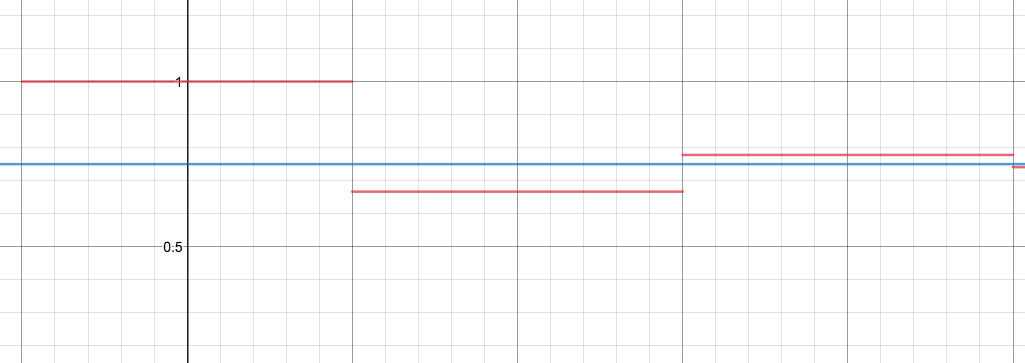
\includegraphics[width=9cm, height=3.5cm]{Images/line2.png}
\end{center}
As we can see here, $\frac{3}{4}$ is graphed as a horizontal line and the points $P_1$, $P_2$, and $P_3$ are graphed as short lines. They represent the partial sums of the series. For example, the line at x=0 is the distance between $P_0$ and $P_1$, the line at x=1 is the distance between $P_1$ and $P_2$, the line at x=2 is the distance between $P_2$ and $P_3$, and so on. We can see that the partial sums start above the horizontal line and then switch between below and above, infinitely. This represents the switch between positive and negative values in the series. The partial sums are growing closer and closer to $\frac{3}{4}$, approaching from above and below. This means that $lim_{k\to\infty}\sum\limits_{k=0}^{\infty} (-\frac{1}{3})^k=\frac{3}{4}$, confirming what we already knew. 
$$\fbox{\textbf{Time for a Quick Break! Fun Fact:} To make a pound of honey, a hive of bees must fly 55,000 miles.}$$
\section*{Predicting the Location of the Third Bee}
This time, instead of the bee returning half or a third of the way, the bee returns a fourth of the way. It flies in the same flight pattern as the other two bees, forming arcs. Since we've seen the series work the same for one-half and one-third when it was substituted in, we can conclude that it'll work the same for one-fourth. 
$$\sum\limits_{k=0}^{\infty} (-\frac{1}{4})^k$$
Now, let's find what it converges to, or what the ultimate location of the bee will be. We can do this by using the geometric series that we derived. We know that a, or the first term, will be 1, and the common ratio, or r, will be $-\frac{1}{4}$.
$$lim_{k\to\infty}\sum\limits_{k=0}^{\infty} (-\frac{1}{4})^k=\frac{1}{1--\frac{1}{4}}=\frac{1}{\frac{5}{4}}=\frac{4}{5}$$
So, the bee ultimately ends up at $\frac{4}{5}$. Let's look at a visual once more.
\begin{center}
    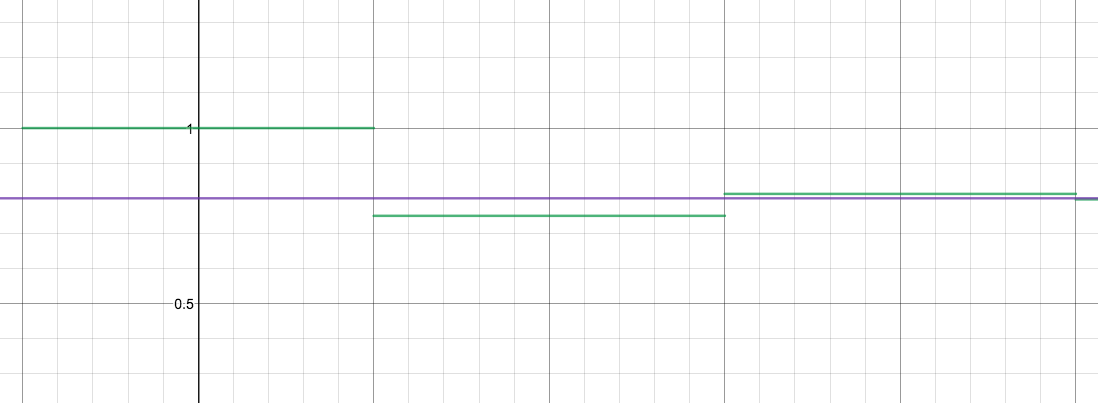
\includegraphics[width=9cm, height=3.5cm]{Images/line3.png}
\end{center}
As we can see here, just as with the other two bees, the horizontal line represents $\frac{4}{5}$, or the bee's ultimate location, and the short lines represent the partial sums of the series. For example, the line at x=0 is the distance between $P_0$ and $P_1$, the line at x=1 is the distance between $P_1$ and $P_2$, the line at x=2 is the distance between $P_2$ and $P_3$, and so on. We can see that the partial sums start above the horizontal line and then switch between below and above, infinitely. This represents the switch between positive and negative values in the series. The partial sums are growing closer and closer to $\frac{4}{5}$, approaching from above and below. This means that $lim_{k\to\infty}\sum\limits_{k=0}^{\infty} (-\frac{1}{4})^k=\frac{4}{5}$, confirming what we already knew.
\section*{Predicting the Location of the Last Bee}
This time, instead of finding the location of the bee that travels one-half, one-third, or one-fourth of the way to each point, we're finding the bee's location when it travels to a general one-kth of the way. Since we've seen the form of the series for one-third and one-fourth of the way work when they were substituted into the the series for one-half, we can do the same thing for one-kth of the way. So, our series would be:
$$\sum\limits_{n=0}^{\infty} (-\frac{1}{k})^n$$
The only thing that's changed about this is that the lower bound and the exponent of the series are in terms of a different variable, n, because we already have a k in the denominator and we don't want our variables getting confused. Now, let's use the geometric series that we derived where the first term, a, equals one, and the common ratio, r, equals $\frac{1}{k}$.
$$\frac{1}{1--\frac{1}{k}}=\frac{1}{\frac{k+1}{k}}=\frac{k}{k+1}$$
So, in the general form, the bee's ultimate location for a bee that travels any fraction of the way back each time can be predicted by $\frac{k}{k+1}$. In this, k is the number in the denominator of the fraction of the way that the bee returned each time. For example, when the bee traveled one-half of the way back each time, its ultimate location was $\frac{2}{2+1}$, or $\frac{2}{3}$. This makes a lot of sense when we look at the ultimate location for every bee that we've looked at so far.
$$\fbox{\textbf{Time for a Quick Break! Fun Fact:} The honey bee is the official insect of Maine.}$$
\section*{Conclusion}
We can use the flight of the bee to better understand the difference between total distance traveled and displacement. In this case, the displacement is a partial sum at any point, which includes the addition of negative values with the positive ones. The total distance traveled would take the absolute value of the general series $\sum\limits_{n=0}^{\infty} (-\frac{1}{k})^n$ and turn it into $\sum\limits_{n=0}^{\infty} (\frac{1}{k})^n$. Each value in this series would be positive and it would sum up to a larger number than displacement. We can look at an example of the bee that returns one-half of the way to see the difference between total distance traveled and displacement. Let's look at the displacement and the total distance traveled at $P_3$. The displacement is $\frac{3}{4}$ and the total distance traveled is $1\frac{3}{4}$, more than 2 times the amount of the displacement! This is just one of many examples that illustrates the difference between total distance traveled and displacement.\\\\
Overall, the behavior of geometric series is interesting to chart, and it can be made even more interesting to explore by studying the path of some happy little bees. 
\end{document}
